\documentclass[border=6pt]{standalone}
\usepackage[utf8]{inputenc}
\usepackage[T1]{fontenc}
\usepackage{varwidth}
\usepackage{tikz}
\usetikzlibrary{calc,backgrounds}
\renewcommand{\familydefault}{\sfdefault}
\tikzset{
  bot/.style={rectangle, rounded corners=6pt, fill=white, draw=black!25, inner sep=5pt, align=left},
  pac/.style={rectangle, rounded corners=6pt, fill=green!12, draw=green!45!black!40, inner sep=5pt, align=left},
}
\begin{document}
\small\hyphenpenalty=10000\exhyphenpenalty=10000
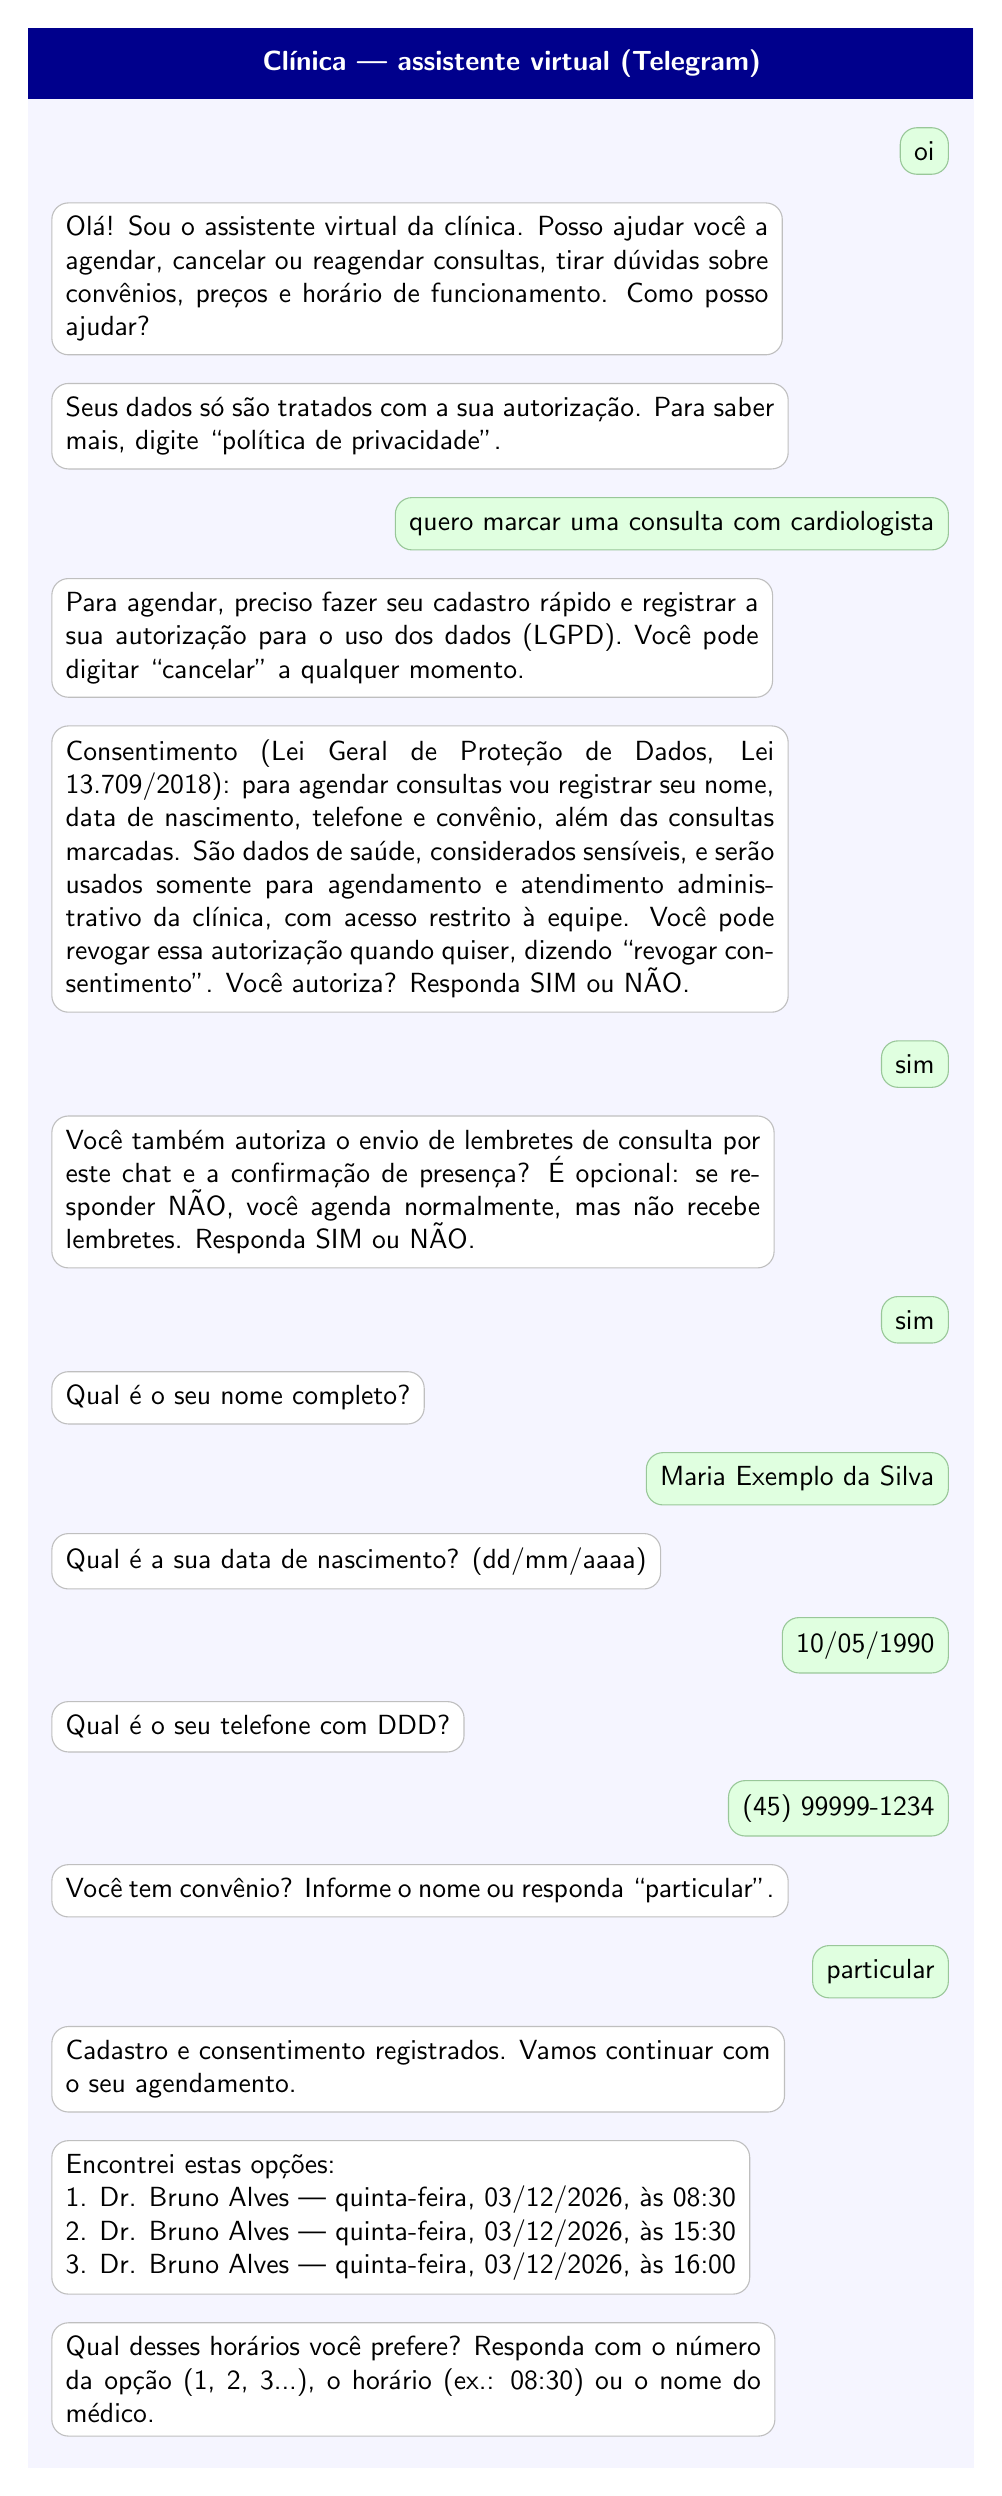
\begin{tikzpicture}
\def\W{12}
\node[anchor=north west, fill=blue!55!black, text=white, minimum width=\W cm, minimum height=0.9cm,
      inner sep=0pt, font=\bfseries] (topo) at (0,0) {\hspace{8pt}Clínica — assistente virtual (Telegram)};
\coordinate (dir) at ({\W-0.3},0);
\coordinate (esq) at (0.3,0);

\path (topo.south) ++(0,-3.5mm) coordinate (c1);
\node[pac, anchor=north east] (m1) at (dir |- c1) {\begin{varwidth}{7.5cm}oi\end{varwidth}};
\path (m1.south) ++(0,-3.5mm) coordinate (c2);
\node[bot, anchor=north west] (m2) at (esq |- c2) {\begin{varwidth}{9cm}Olá! Sou o assistente virtual da clínica. Posso ajudar você a agendar, cancelar ou reagendar consultas, tirar dúvidas sobre convênios, preços e horário de funcionamento. Como posso ajudar?\end{varwidth}};
\path (m2.south) ++(0,-3.5mm) coordinate (c3);
\node[bot, anchor=north west] (m3) at (esq |- c3) {\begin{varwidth}{9cm}Seus dados só são tratados com a sua autorização. Para saber mais, digite ``política de privacidade''.\end{varwidth}};
\path (m3.south) ++(0,-3.5mm) coordinate (c4);
\node[pac, anchor=north east] (m4) at (dir |- c4) {\begin{varwidth}{7.5cm}quero marcar uma consulta com cardiologista\end{varwidth}};
\path (m4.south) ++(0,-3.5mm) coordinate (c5);
\node[bot, anchor=north west] (m5) at (esq |- c5) {\begin{varwidth}{9cm}Para agendar, preciso fazer seu cadastro rápido e registrar a sua autorização para o uso dos dados (LGPD). Você pode digitar ``cancelar'' a qualquer momento.\end{varwidth}};
\path (m5.south) ++(0,-3.5mm) coordinate (c6);
\node[bot, anchor=north west] (m6) at (esq |- c6) {\begin{varwidth}{9cm}Consentimento (Lei Geral de Proteção de Dados, Lei 13.709/2018): para agendar consultas vou registrar seu nome, data de nascimento, telefone e convênio, além das consultas marcadas. São dados de saúde, considerados sensíveis, e serão usados somente para agendamento e atendimento administrativo da clínica, com acesso restrito à equipe. Você pode revogar essa autorização quando quiser, dizendo ``revogar consentimento''. Você autoriza? Responda SIM ou NÃO.\end{varwidth}};
\path (m6.south) ++(0,-3.5mm) coordinate (c7);
\node[pac, anchor=north east] (m7) at (dir |- c7) {\begin{varwidth}{7.5cm}sim\end{varwidth}};
\path (m7.south) ++(0,-3.5mm) coordinate (c8);
\node[bot, anchor=north west] (m8) at (esq |- c8) {\begin{varwidth}{9cm}Você também autoriza o envio de lembretes de consulta por este chat e a confirmação de presença? É opcional: se responder NÃO, você agenda normalmente, mas não recebe lembretes. Responda SIM ou NÃO.\end{varwidth}};
\path (m8.south) ++(0,-3.5mm) coordinate (c9);
\node[pac, anchor=north east] (m9) at (dir |- c9) {\begin{varwidth}{7.5cm}sim\end{varwidth}};
\path (m9.south) ++(0,-3.5mm) coordinate (c10);
\node[bot, anchor=north west] (m10) at (esq |- c10) {\begin{varwidth}{9cm}Qual é o seu nome completo?\end{varwidth}};
\path (m10.south) ++(0,-3.5mm) coordinate (c11);
\node[pac, anchor=north east] (m11) at (dir |- c11) {\begin{varwidth}{7.5cm}Maria Exemplo da Silva\end{varwidth}};
\path (m11.south) ++(0,-3.5mm) coordinate (c12);
\node[bot, anchor=north west] (m12) at (esq |- c12) {\begin{varwidth}{9cm}Qual é a sua data de nascimento? (dd/mm/aaaa)\end{varwidth}};
\path (m12.south) ++(0,-3.5mm) coordinate (c13);
\node[pac, anchor=north east] (m13) at (dir |- c13) {\begin{varwidth}{7.5cm}10/05/1990\end{varwidth}};
\path (m13.south) ++(0,-3.5mm) coordinate (c14);
\node[bot, anchor=north west] (m14) at (esq |- c14) {\begin{varwidth}{9cm}Qual é o seu telefone com DDD?\end{varwidth}};
\path (m14.south) ++(0,-3.5mm) coordinate (c15);
\node[pac, anchor=north east] (m15) at (dir |- c15) {\begin{varwidth}{7.5cm}(45) 99999-1234\end{varwidth}};
\path (m15.south) ++(0,-3.5mm) coordinate (c16);
\node[bot, anchor=north west] (m16) at (esq |- c16) {\begin{varwidth}{9cm}Você tem convênio? Informe o nome ou responda ``particular''.\end{varwidth}};
\path (m16.south) ++(0,-3.5mm) coordinate (c17);
\node[pac, anchor=north east] (m17) at (dir |- c17) {\begin{varwidth}{7.5cm}particular\end{varwidth}};
\path (m17.south) ++(0,-3.5mm) coordinate (c18);
\node[bot, anchor=north west] (m18) at (esq |- c18) {\begin{varwidth}{9cm}Cadastro e consentimento registrados. Vamos continuar com o seu agendamento.\end{varwidth}};
\path (m18.south) ++(0,-3.5mm) coordinate (c19);
\node[bot, anchor=north west] (m19) at (esq |- c19) {\begin{varwidth}{9cm}Encontrei estas opções:\\1. Dr. Bruno Alves — quinta-feira, 03/12/2026, às 08:30\\2. Dr. Bruno Alves — quinta-feira, 03/12/2026, às 15:30\\3. Dr. Bruno Alves — quinta-feira, 03/12/2026, às 16:00\end{varwidth}};
\path (m19.south) ++(0,-3.5mm) coordinate (c20);
\node[bot, anchor=north west] (m20) at (esq |- c20) {\begin{varwidth}{9cm}Qual desses horários você prefere? Responda com o número da opção (1, 2, 3...), o horário (ex.: 08:30) ou o nome do médico.\end{varwidth}};
\path (m20.south) ++(0,-4mm) coordinate (fim);
\begin{scope}[on background layer]
  \fill[blue!4] (topo.north west) rectangle (topo.east |- fim);
\end{scope}
\end{tikzpicture}
\end{document}
